\chapter{Analysis techniques}

\section{General strategy for searching for four top quarks}

The LHC has been said to be a ``top factory'' due to the large cross sections for \ttbar production at 8 TeV and 13 TeV, 253~pb and 831~pb respectively. Hence most analyses within the CMS collaboration which work on top quark physics study \ttbar production. Each of the top quarks will decay to a W boson and a b quark and the final state of the process in the detector is defined by whether the W boson decays leptonically into a lepton and neutrino or hadronically into two quark jets. The standard strategy is to require two b-jets to be present in the event and 0, 1, 2 leptons depending on the final state defined as \emph{all-hadronic}, \emph{semi-leptonic} and emph{dileptonic} respectively where 6, 4 or 2 jets are required. 

\begin{figure}[ht!]
\centering
    \includegraphics[width=0.5\textwidth]{images/Analysis/Ttbar_decay_channels.png}
    \caption{The possible decay channels for \ttbar production}
    \label{fig:ttbarDecay}
\end{figure}
%picture from wiki By Nazar Bartosik - http://bartosik.pp.ua/hep_sketches/tt_decay_channels, CC BY 4.0, https://commons.wikimedia.org/w/index.php?curid=49739344

Each selection of b-jets, leptons and total number of jets in the event will not be $100\%$ efficient which means not all \ttbar events will be captured within the selection. As the rate of \ttbar production is so high at the LHC, this is satisfactory as the total number of events is still high enough to have statistically relevant studies.\\

The strategy for selecting \tttt events while suppressing the selection of background processes is similar to the \ttbar selection but with the selection of additional two jets. The small cross section for \tttt production, 1.3~fb at 8~TeV and $\approx$9~fb at 13~TeV dictates the selection. It would be preferential to require 4 b-jets in the selection to obtain the highest signal to background ratio, however as b-tagging is $\approx70\%$ efficient, this would have a detrimental effect on the overall amount of \tttt found in the selection due to some b-jets not being identified correctly or being within the acceptance of the detector. Similarly, it is not possible to require the total number of jets in a \tttt final state as some of the jets may not be within the acceptance of the detector. However, it will be discussed in section~\ref{sec:Categorisation} how a looser selection can be used to an advance to constrain the main background process.

This thesis will mainly focus on the single lepton channel where only single muon and single electron final states are considered. As can be seen from~\ref{fig:ttttDecay}, the single lepton channel represents the largest branching ratio or four top quark decay channel. The dilepton channel, which has the second largest branching ratio will also briefly be discussed in chapter~\ref{c:Run2} as it was combined with the single lepton channel to achieve an increased sensitivity on the analysis. In the dilepton channel only final states with muons and electrons were considered.

\begin{figure}[ht!]
\centering
    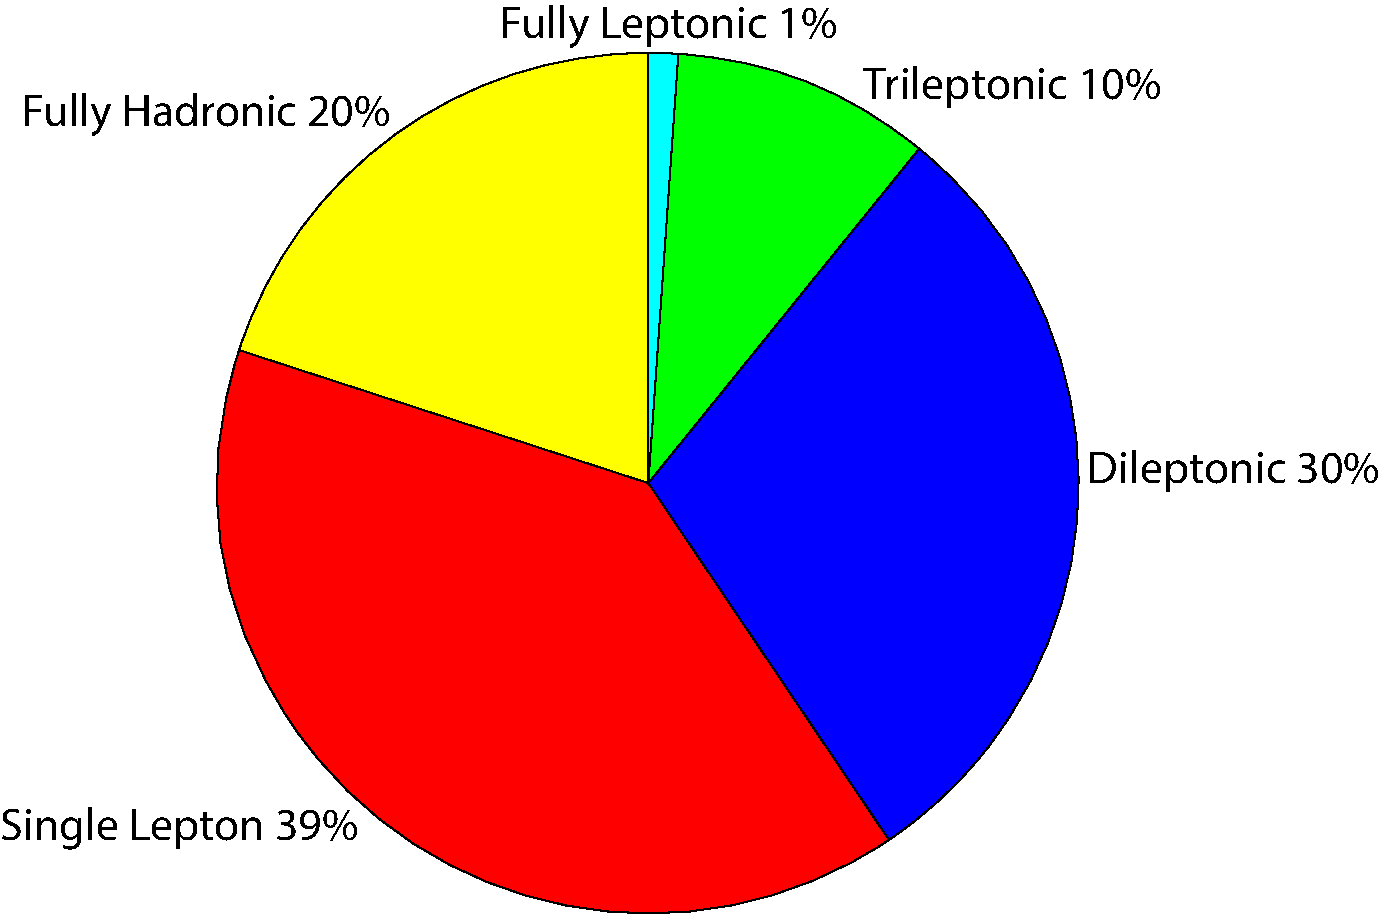
\includegraphics[width=0.5\textwidth]{images/Analysis/FourTopBR.pdf}
    \caption{The possible decay channels for \tttt production}
    \label{fig:ttttDecay}
\end{figure}




\section{Calibrations of the simulation}
\label{sec:Calibrations}
Many of the parameters which go into making simulation for each particle physics process are not precisely known therefore they are tuned to produce the simulation which best matches the data observed. This simulation will still have discrepancies from data which can be measured and accounted for by producing \emph{scale factors} which are combined and adjust the weight of each event in the simulation such that the overall distributions more closely matches data. 


\subsection{Pileup modelling}
\label{sec:pile-up}
The distribution of the number of primary vertices varies between data and simulation. This can be taken into account by looking at the number of events for each number of primary vertices in data and simulation and applying the scale factor, $SF_{PU}\left( i \right)$ to simulation, where \emph{i} is the number of vertices.

\begin{equation}
SF_{PU}\left( i \right) = \frac{N_{events}^{Data}}{  N_{events}^{simu}} 
\label{eqn:PUSF}
\end{equation}

\subsection{b tag modelling}

There are significant differences between b tagging efficiencies measured by CMS in data and the efficiencies as measured in simulation as it is difficult to simulate the fragmentation and hadronisation of b-quarks. 
The b-tagging efficiencies are measured for each of the CSVL, CSVM, and CSVT working points in bins of \pt and $\eta$. Depending on which working point was used in an analysis a scale factor, $SF(\eta, P_{T})_{i}$,  can be applied to the simulation for each jet which is dependent on the \pt, $\eta$ and flavour of the jet, shown in equation~\ref{eqn:sfbtagnorm}, where $\epsilon(\eta , \pt)^{data}_{i}$ is the efficiency for correctly identifying a b-jet in data and $\epsilon(\eta , \pt)^{simulation}_{i}$ is the efficiency for correctly identifying a b-jet in simulation.

\begin{centering}
\begin{equation}
SF(\eta, P_{T})_{i} = \frac{\epsilon(\eta , \pt)^{data}_{i}}{\epsilon(\eta , \pt)^{simulation}_{i}}
\label{eqn:sfbtagnorm}
\end{equation}
\end{centering}
Separate scale factors are defined by b and light (u, d, s, g) jets. Scale factors for c jets are taken to be the same as for b jets. A weight, $\omega_{btag}$ is applied to simulated events in order to correct for the expected difference between the efficiency in data and simulation. The method proceeds by defining the probability of an event in simulation producing a given number of tagged and untagged jets, P(MC),:

\begin{centering}
\begin{equation}
P(MC) = \prod_{tagged jets}\epsilon_{i} \times \prod_{untagged jets}(1- \epsilon_{i})
\end{equation}
\end{centering}
where $\epsilon_{i}$ is the efficiency of tagging a jet flavour $i$ with the CSV criterion. While the probability of an event in data producing a given number of tagged and untagged jets, P(DATA), is defined as follows:


\begin{centering}
\begin{equation}
P(DATA) = \prod_{tagged jets}SF_{i}\cdot\epsilon_{i} \times \prod_{untagged jets}(1- SF_{i}\cdot\epsilon_{i})
\end{equation}
\end{centering}
where SF is the appropriate scale factor for a jet of flavour $i$. 

An overall weight to be applied to each event depending on the jet content can be derived from these scale factors using the formula in~\ref{eqn:weightbtagnorm}. This weight, $\omega_{btag}$, must be applied to the selected simulation events in order to predict the correct event yield in data.

\begin{centering}
\begin{equation}
 \omega_{btag} = \frac{P(DATA)}{P(MC)}
 \label{eqn:weightbtagnorm}
\end{equation}
\end{centering}


Alternatively, the measurements at each working point can be used to fit the shape of the CSV distribution and provide scale factors in bins of \pt and $\eta$ for each jet flavour. Therefore the scale factors for each jet can be derived from the \pt and $\eta$, CSV discriminator value and for each jet flavour as seen in equation~\ref{eqn:btagcsv}. For this method, the jet flavours are defined as heavy for bottom quarks and light for u, s, d, g whilst c-quarks are given $\textrm{SF} = 1$. Further details of the CSV reshaping can be found in Ref.~\cite{CMS-NOTE-2013-130}.

\begin{equation}
\textrm{SFjet}_{\textrm{B}} \left(\textrm{CSV},\pt,\eta \right) = \frac{\textrm{Data} - \textrm{MC}_{\textrm{A}}}{\textrm{MC}_{\textrm{B}}} ~~;~~ \textrm{A, B = heavy flavour, light flavour or vice versa}
\label{eqn:btagcsv}
\end{equation}

An event weight can be derived by taking the product of the per-jet scale factors as seen in equation~\ref{eqn:btagcsvtot}.

\begin{equation}
\textrm{SF}_{\textrm{total}} = \prod_{i}^{\njets}\textrm{SFjet}_{i}
\label{eqn:btagcsvtot}
\end{equation}

\subsection{Heavy flavour jet modelling}
There is a discrepancy between data and simulation in the distribution of the number of b-tagged jets (\nbtags) at higher numbers of b-tags which suggests that the amount of heavy flavour jets in \ttbar events is incorrectly simulated. The extra jets can come from processes such as gluon splitting pair-producing \bbbar in \ttbar events. These \ttbb events are most likely to resemble to features of the \tttt signal events and so it is essential that the proportion of them in simulation is correctly modelled.
The ratio of $R=$\heavyflavour was measured by CMS to be $2.2 \pm 0.3 \left( \textrm{stat.} \right) \pm 0.5 \left(\textrm{sys.} \right)\% $ ~\cite{Khachatryan2015132} at $\sqrt{s} =$ 8~TeV and to be $2.2 \pm 0.3 \left( \textrm{stat.} \right) \pm 0.6 \left(\textrm{sys.} \right)\% $ ~\cite{CMS-PAS-TOP-16-010} at $\sqrt{s} =$ 13~TeV. To incorporate this ratio into the analysis, the MC truth information of the \ttbar$+$jets (MC) sample is used to split the sample into \ttbb, \ttcc and \ttll, where l denotes light quarks and gluons (\cPqu, \cPqd, \cPqs, \cPg). Weights are applied to each sub-sample to match the measured ratio whilst preserving the total number of \ttbar events.

\subsection{Lepton modelling}
Due to a difference between data and simulation in the efficiency of lepton identification, isolation, reconstruction and triggering, a weight is applied to events which is dependent on the selected leptons $\eta$, $\pt$ and lepton flavour. The scale factors for each source of efficiency are designed to be multiplicative and the final event weight can be found in equation~\ref{eqn:leptonW}

\begin{equation}
\omega_{lepton} = SF_{iso}\times SF_{id}\times SF_{reco}\times SF_{trig}
\label{eqn:leptonW}
\end{equation}

\subsection{Top \pt reweighting}

There is a known problem in the modelling of the top quark \pt spectrum where the top quarks found in data appear tend to be lower in \pt than simulation. A scale factor can be derived as a function of the \pt of the top as generated in the simulation before being reconstructed in the detector. The event weight is shown in equation~\ref{eqn:topptW}

\begin{equation}
\omega_{topPt} = SF_{top}\times SF_{anti-top}
\label{eqn:topptW}
\end{equation}

\subsection{Jet multiplicity modelling}
Good modelling of the jet multiplicity distribution up to a large number of jets (up to fifteen jets) in the main \ttbar background is highly important for this analysis because as the number of jets increase the signal to background ratio increases. Hence, the higher \njets multiplicity categories mentioned in section~\ref{sec:Cats} are where the highest sensitivity in separating the signal \tttt process and the background \ttbar process. It is essential that \ttbar is well modelled in this high jet multiplicity region. 
Particularly at 13 TeV the simulation was larger than data in the higher \njets bins. The value of $\alpha_S$ in the \ttbar Powheg+Pythia8 sample used in the~\ref{c:Run2} analysis is 0.137, however the best tune was observed by the TOP-PAG to have a value of $\alpha_S=0.113^{+0.012}_{0.010}$. A scale factor was derived by CMS in order to improve the modelling of the \njets distribution. 

\section{Multi-jet background estimation}
\label{sec:QCDbackground}
The presence of multi-jet events within the signal region defined by the baseline selection is investigated in this section. It is rare for multi-jet events to have a highly energetic undetectable particle\fixme{why?}. Therefore, the $\MET$ distributions for multi-jet events typically peak at low values, not necessarily at zero as some jets maybe outside of the acceptance of the detector or mismeasured. Due to the small number of events which pass the selection and the difficulty in simulating QCD events, it is not possible to use multi-jet simulation to estimate this background. In this case, a data-driven method known as the \fxnote*{ref?}{ABCD method} may be used. This method proceeds by selecting two uncorrelated variables from the object or baseline selection and defining three control regions (A,B,C) and one signal region, D, in the 2-dimensional phase space of these variables. The event variable \MET and the lepton variable RelIso were selected as they are \fxnote*{uncorrelated proof??}{uncorrelated} and the defined regions are shown below. \fxnote*{be precise}{Trigger requirements place an upper bound on the RelIso which restricts the region choice}.\\

\fixme{advantages of ABCD/assumptions}
\fxnote{Residual dependence on simulation}

\section{Multi-variate analysis techniques}
\subsection{Boosted Decision Trees}
\label{sec:BDT}


\subsection{Reconstruction of hadronic top quarks}

\subsection{Event-level BDT}

\section{Limit setting}

\subsection{Categorisation}
\label{sec:Cats}




